\documentclass[hidelinks]{ctexart}

\usepackage[sensei=陈向军/刘明辉,gakka=原子物理学,section=Bunshibutsurigaku,gakkabbr=AP]{styles/kurisu}
\usepackage{van-de-la-illinoise}
\sisetup{range-phrase=\sim}

\begin{document}

\section{分子\textsf{エネルギー}準位} % (fold)
\label{sec:分子エネルギー準位}

\subsection{分子能级结构与光谱概述} % (fold)
\label{sub:分子能级结构与光谱概述}

\newpoint{分子平衡构型} 原子核在分子中的位置基本固定. 中性$\ce{H2}$分子的平衡核间距为$\SI{0.074}{\nano\meter}$, 中性$\ce{O2}$分子的平衡核间距为$\SI{0.121}{\nano\meter}$.
\newpoint{化学键} 当原子结合形成分子时, 内壳层电子几乎不受影响, 仍然局域在每个原子上. 外壳层价电子则分布在整个分子中. 价电子的电荷分布提供了分子形成的相互作用力, 谓\gloss{化学键}.
\newpoint{}从质心建立坐标, 可消除分子的平动能级. 转动能级和振动能级时量子化的.

\subsubsection{能量估算} % (fold)
\label{ssub:能量估算}

\newpoint{}价电子激发态能量估算,
\[ p_e \approx \frac{\hbar}{R_0} \Rightarrow E_e = \frac{p_e^2}{2m_e} \approx \frac{\hbar^2}{2m_e R_0^2}. \]
当$R_0 = \SI{0.1}{\nano\meter}$, 有$E_e \approx \SIrange{1}{10}{\eV}$. 和原子光谱能量相当, 在紫外或可见光区.
\newpoint{}核运动引入振动和转动能级. 设原子核之间的力为简谐力, 电子和原子核振动的频率分别为
\[ \nu_e = \rec{2\pi}\sqrt{\frac{k}{m_e}},\quad \nu_N = \rec{2\pi}\sqrt{\frac{k}{M}}. \]
相应的能量比为
\[ \frac{h\nu_e}{h\nu_N} \approx \sqrt{\frac{M}{m_e}} \Rightarrow E_\nu \approx 10^{-1}E_e \approx \SIrange{e-2}{e-1}{\eV}. \]
\newpoint{}核转动的能量估计,
\[ E_r = \frac{L^2}{2I} = \frac{L^2}{MR_0^2}, \]
取$L\approx \hbar$, 有
\[ E_r \approx \frac{\hbar^2}{MR_0^2} \approx \frac{m_e}{M}E_e \approx 10^{-4}E_e \approx \SIrange{e-4}{e-3}{\eV}. \]
\newpoint{}因此双原子分子的能级是电子能级上叠加振动能级, 再叠加转动能级. 纯转动光谱在远红外区, 即毫米/厘米量级. 纯振动光谱在近红外区, 即微米量级. 在两个电子能级之间的跃迁在可见光/紫外区, 由于必然伴随转动/振动能级跃迁, 将形成光谱带系.

% subsubsection 能量估算 (end)

% subsection 分子能级结构与光谱概述 (end)

\subsection{分子的化学键} % (fold)
\label{sub:分子的化学键}

\newpoint{}组成分子/晶体的相邻原子之间有相互吸引作用, 谓化学键.
\newpoint{}碱金属最外层皆为单个s电子. 卤族元素最外层有一个p电子空位.
\newpoint{电子亲合势} 基态中性原子俘获一个电子称为一价负离子而释放出的能量. 亲合势越大, 获得电子的倾向越强.
\newpoint{}$\ce{Nacl}$由价电子的转移形成离子键而得到. \gloss{离子键}由价电子的转移形成.
\newpoint{}$\ce{Cl2}$由价电子的共用形成共价键而得到. \gloss{共价键}由价电子的共用形成.
\newpoint{}电负性差别大的原子形成分子是以离子键结合. 电负性差别小的原子以共价键结合.

\subsubsection{离子键} % (fold)
\label{ssub:离子键}

\newpoint{}$\ce{Na}$的电离能为$\SI{5.14}{\eV}$, $\ce{Cl}$的电子亲合势为$\SI{3.62}{\eV}$, 从而$\ce{Na + Cl -> Na+ + Cl-}$需要花费$5.14-3.62 = \SI{1.52}{\eV}$的能量.
\newpoint{}$\ce{NaCl}$分子的能量随间距上升先减后增, 在$R_0 = \SI{0.24}{\nano\meter}$时有最小值$\SI{-4.26}{\eV}$. 这是二者的\gloss{结合能}, 也是$\ce{NaCl}$分解为$\ce{Na}$和$\ce{Cl}$原子时的\gloss{解离能}.
\newpoint{}$R\rightarrow 0$时Pauli斥力占主导作用. $R\rightarrow \infty$时能量曲线收敛于$\SI{1.52}{\eV}$.
\newpoint{}离子键形成的分子通常为极性分子.

% subsubsection 离子键 (end)

\subsubsection{共价键} % (fold)
\label{ssub:共价键}

\newpoint{}考虑$\ce{H2+}$分子离子, 体系的Hamiltonian为
\[ \hat H = -\frac{\hbar^2}{2m_e} \laplacian - \frac{e^2}{4\pi\epsilon_0 r_a} - \frac{e^2}{4\pi\epsilon_0 r_b} + \frac{e^2}{4\pi\epsilon_0 R}. \]
\newpoint{}如果仅考虑基态, 极端情形下电子在质子$a$附近运动,
\[ \hat H \approx -\frac{\hbar^2}{2m_e}\laplacian - \frac{e^2}{4\pi\epsilon_0 r_a},\quad u\+_1s_\pare{r_a} = \sqrt{\rec{\pi a_0^3}}e^{-r_a/a_0}. \]
或者在$b$附近运动,
\[ \hat H \approx -\frac{\hbar^2}{2m_e}\laplacian - \frac{e^2}{4\pi\epsilon_0 r_b},\quad u\+_1s_\pare{r_b} = \sqrt{\rec{\pi a_0^3}}e^{-r_b/a_0}. \]
\newpoint{}分子轨道表示为原子轨道的线性组合(LCAO)近似下,
\[ \psi = c_a \psi\+_1s_\pare{r_a} + c_b \psi\+_1s_\pare{r_b}. \]
利用变分法,
\begin{align*}
    \psi_g = \rec{\sqrt{2+2S}}\brac{u\+_1s_\pare{r_a} + u\+_1s_\pare{r_b}},\quad E_g = \frac{\alpha + \beta}{1+S}, \\
    \psi_u = \rec{\sqrt{2-2S}}\brac{u\+_1s_\pare{r_a} - u\+_1s_\pare{r_b}},\quad E_u = \frac{\alpha - \beta}{1-S}.
\end{align*}
Coulomb积分为
\[ \alpha = \bra{u\+_1s_}\hat H \ket{u\+_1s_} = E\+_1s_ + \frac{e^2}{4\pi\epsilon_0 R} - \int \frac{e^2\abs{u\+_1s_\pare{r_a}}^2}{4\pi\epsilon_0 r_b}\,\rd{\tau}. \]
交换积分为
\[ \beta = \int u\+_1s_\pare{r_a}\hat H u\+_1s_\pare{r_b}\,\rd{\tau}. \]
重叠积分为
\[ S = \int u\+_1s_\pare{r_a} u\+_1s_\pare{r_b}\,\rd{\tau}. \]
$\psi_g$在$R_0 = \SI{0.132}{\nano\meter}$处有极小, $E_g\pare{R_0} = \SI{-15.37}{\eV}$. 反键轨道$\psi_u$的势能曲线随$R$增大而单调下降. 成键的关键在于交换积分
\[ \beta = \int u\+_1s_\pare{r_a}\hat H u\+_1s_\pare{r_b}\,\rd{\tau} < 0. \]
令$S=0$, 则
\begin{align*}
    \psi_g &= \rec{\sqrt{2}}\brac{u\+_1s_\pare{r_a} + u\+_1s_\pare{r_b}}, \\
    \psi_u &= \rec{\sqrt{2}}\brac{u\+_1s_\pare{r_a} - u\+_1s_\pare{r_b}}, \\
    \abs{\psi_{g}}^2 &= \half \brac{\abs{u\+_1s_\pare{r_a}}^2 + \abs{u\+_1s_\pare{r_b}}^2 + 2u\+_1s_\pare{r_a}u\+_1s_\pare{r_b}}, \\
    \abs{\psi_{u}}^2 &= \half \brac{\abs{u\+_1s_\pare{r_a}}^2 + \abs{u\+_1s_\pare{r_b}}^2 - 2u\+_1s_\pare{r_a}u\+_1s_\pare{r_b}}.
\end{align*}
故成键轨道电子在中间的概率增加, 反键轨道电子在中间的概率极小.
\par
氢原子的精确数据为
\[ R_0 = \SI{0.106}{\nano\meter},\quad E_g = E\+_1s_ - \SI{2.79}{\eV},\quad \alpha = \pare{0.97\sim 1}E\+_1s_. \]
令$S=0$, 则
\[ \begin{cases}
    E_g = E\+_1s_ + \beta, \\
    E_u = E\+_1s_ - \beta.
\end{cases} \]
\begin{center}
    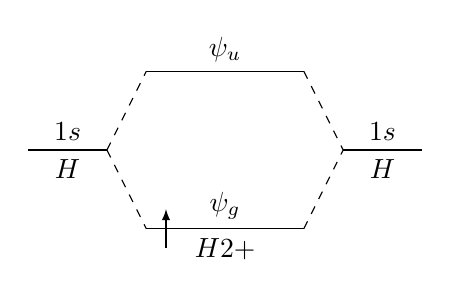
\begin{tikzpicture}[yscale=1]
        \draw (-2.5,0) -- (-1.5,0) node[midway,below] {$\ce{H}$} node[midway,above] {$\ce{1s}$};
        \draw (1.5,0) -- (2.5,0) node[midway,below] {$\ce{H}$} node[midway,above] {$\ce{1s}$};
        \draw (-1,1) -- (1,1) node[midway,above] {$\psi_u$};
        \draw (-1,-1) -- (1,-1) node[midway,above] {$\psi_g$} node[midway,below] {$\ce{H2+}$};
        \draw[-latex] (-0.75,-1.25) -- (-0.75,-0.75);
        \draw[dashed] (-1.5,0) -- (-1,1) (-1.5,0) -- (-1,-1) (1,1) -- (1.5,0) (1,-1) -- (1.5,0);
    \end{tikzpicture}
\end{center}
如果在成键轨道上放入两个电子, 则
\[ R_0 = \SI{0.074}{\nano\meter},\quad E_g = E\+_1s_ - \SI{4.7}{\eV}. \]

% subsubsection 共价键 (end)

% subsection 分子的化学键 (end)

\subsection{双原子分子的能级和光谱} % (fold)
\label{sub:双原子分子的能级和光谱}

\subsubsection{Born-Oppenheimer近似} % (fold)
\label{ssub:born_oppenheimer近似}

设双原子分子由$N$个电子和两个核电子数分别为$Z_a$和$Z_b$的原子核组成, 体系的Hamiltonian为
\[ \hat H = \sum_{i=1}^N\pare{-\frac{\hbar^2}{2m_e}\laplacian_i} + \pare{-\frac{\hbar^2}{2M_a}\laplacian_a - \frac{\hbar^2}{2M_b}\laplacian_b} + \sum_{i=1}^N\pare{-\frac{Z_a e^2}{4\pi\epsilon_0 r_{ai}} - \frac{Z_b e^2}{4\pi\epsilon_0 r_{bi}}} + \sum_{i<j=1}^N \frac{e^2}{4\pi\epsilon_0 r_{ij}} +\frac{Z_aZ_b e^2}{4\pi\epsilon_0 R}. \]
处理电子运动时假设两电子间距保持不变, 即
\[ \hat H = \sum_{i=1}^N\pare{-\frac{\hbar^2}{2m_e}\laplacian_i} +\sum_{i=1}^N\pare{-\frac{Z_a e^2}{4\pi\epsilon_0 r_{ai}} - \frac{Z_b e^2}{4\pi\epsilon_0 r_{bi}}} + \sum_{i<j=1}^N \frac{e^2}{4\pi\epsilon_0 r_{ij}} + \frac{Z_aZ_b e^2}{4\pi\epsilon_0 R}. \]
双原子分子的电子运动的Schr\"odinger方程为
\[ \brac{\hat H_e + V_{NN}}\Psi_e = U\Psi_e, \]
其中
\[ \hat H_e = \sum_{i=1}^N\pare{-\frac{\hbar^2}{2m_e}\laplacian_i} +\sum_{i=1}^N\pare{-\frac{Z_a e^2}{4\pi\epsilon_0 r_{ai}} - \frac{Z_b e^2}{4\pi\epsilon_0 r_{bi}}} + \sum_{i<j=1}^N \frac{e^2}{4\pi\epsilon_0 r_{ij}} \]
而
\[ V_{NN} = \frac{Z_aZ_b e^2}{4\pi\epsilon_0 R}. \]
减去$V_{NN}$后可得
\[ \hat H_e \Psi_e = E_e \Psi_e,\quad E_e = U - V_{NN}. \]
而核运动方程为
\[ \hat H_N \Phi_N = E\Phi_N. \]
其中
\[ \hat H_N = \pare{-\frac{\hbar^2}{2M_a}\laplacian_a - \frac{\hbar^2}{2M_b}\laplacian_b} + U\pare{R}, \]
$E$是分子的总能量, $\Phi_N$是核运动的波函数.
\[ E = E_e + E_\nu + E_r. \]

% subsubsection born_oppenheimer近似 (end)

\subsubsection{转动能级和转动光谱} % (fold)
\label{ssub:转动能级和转动光谱}

相对质心的转动惯量为
\[ I = m_a r_a^2 + m_b r_b^2,\quad m_a r_a =  m_b r_b,\quad R_0 = r_a + r_b \Rightarrow I = \mu R_0^2,\quad \mu = \frac{m_am_b}{m_a + m_b}. \]
转动能为
\[ E_r = \half I\omega^2 = \frac{L^2}{2I},\quad L = I\omega = \mu R_0^2 \omega. \]
等效粒子的Schr\"odinger方程为
\[ -\frac{\hbar}{2\mu}\laplacian \psi_r = E_r \psi_r. \]
采用球极坐标,
\[ -\hbar^2 \brac{\rec{\sin\theta}\+D\theta D{} \pare{\sin \theta \+D\theta D{}} + \rec{\sin^2\theta}\+D{\phi^2}D{^2}}\psi_r = \lambda \psi_r. \]
其中$\lambda = 2IE_r$. 本征函数为球谐函数,
\[ \hat L^2 \psi_r = \lambda \psi_r \Rightarrow \psi_r = Y_{J,M_J}\pare{\theta,\phi}. \]
本征值
\[ \lambda = L^2 = J\pare{J+1}\hbar^2,\quad J = 0,1,2,\cdots. \]
刚性转子的转动能
\[ E_r = E_J = \frac{L^2}{2I} = \frac{\hbar^2}{2I}J\pare{J+1}. \]
两个转动能的能级间隔为
\[ \Delta E_J = E_J - E_{J-1} = \frac{\hbar^2}{2I}\brac{J\pare{J+1} - \pare{J-1}J} = \frac{\hbar^2}{I}J. \]

\paragraph{纯转动光谱} % (fold)
\label{par:纯转动光谱}

电偶极跃迁的选择定则为
\[ \Delta J = \pm 1. \]
转动只能在相邻的能级跃迁, 相应的谱线波数为
\[ \resumath{\tilde{\nu}_J = \frac{E_J - E_{J-1}}{hc} = 2BJ.} \]
其中
\[ \resumath{B = \frac{\hbar}{4\pi Ic} = \frac{\hbar}{4\pi \mu R_0^2 c}.} \]
谓\gloss{转动常数}.
\begin{ex}
    纯转动的吸收光谱, $J=1\leftarrow J=0$波数为$2B$, $J=2 \leftarrow J=1$波数为$4B$.
\end{ex}
\newpoint{}谱线大致等差排列, 由
\[ 2B = \frac{2\hbar}{4\pi\mu R_0^2 c} \]
可得分子的平衡构型.
\newpoint{}热平衡时不同转动能级的分子数分布为
\[ N_i \propto e^{-E_i/k\+_B_T}. \]
转动的能级间隔为
\[ \Delta E = 2Bhc \sim \SI{5e-3}{\eV}. \]
常温下$k\+_B_T \sim \SI{2.5e-2}{\eV}$.

% paragraph 纯转动光谱 (end)

\paragraph{离心畸变修正} % (fold)
\label{par:离心畸变修正}

用抛物线近似势能曲线, 原子核之间近似受到一弹性力
\[ f = -k\pare{R-R_0}, \]
有
\[ \mu \omega^2 R = k\pare{R-R_0}, \]
从而
\[ R-R_0 = \frac{\mu \omega^2 R}{k} = \frac{L^2}{\mu k R^2} \approx \frac{L^2}{\mu k R_0^3}. \]
非刚性转子的能量除了转动能外还应加上弹性势能,
\[ \begin{cases}
    \displaystyle E_J = \frac{L^2}{2\mu R^2} + \half k\pare{R-R_0}^2, \\[.5em]
    \displaystyle R-R_0 = \frac{\mu \omega^2 R}{k} = \frac{L^2}{\mu kR^3} = \frac{L^2}{\mu k R_0^3}.
\end{cases} \]
从而
\[ E_J \approx \frac{L^2}{2\mu R_0^2}\pare{1+\frac{L^2}{\mu kR_0^4}}^{-2} + \half k\pare{\frac{L^2}{\mu kR_0^3}}^2 \approx \frac{L^2}{2\mu R_0^2} - \frac{L^4}{2\mu^2 k R_0^6}. \]
代入$L^2 = J\pare{J+1}\hbar^2$, 有
\[ \resumath{E_J = hc \brac{BJ\pare{J+1} - DJ^2\pare{J+1}^2}.} \]
得
\[ B = \frac{\hbar}{4\pi\mu R_0^2 c},\quad D = \frac{\hbar^3}{4\pi k \mu^2 R_0^6 c}. \]
其中
\[ B = \frac{\hbar}{4\pi \mu R_0^2 c},\quad D = \frac{\hbar^3}{4\pi k\mu^2 R_0^6 c}. \]
从而$J\leftarrow J-1$的吸收波数为
\[ \resumath{\tilde{\nu}_J = \frac{E_J - E_{J-1}}{hc} = 2BJ - 4DJ^3.} \]
相邻谱线的间隔为
\[ \resumath{\Delta\tilde{\nu} = \tilde{\nu}_J - \tilde{\nu}_{J-1} = 2B - 4D\pare{3J^2 - 3J+1}.} \]

% paragraph 离心畸变修正 (end)

% subsubsection 转动能级和转动光谱 (end)

\subsubsection{振动能级和振动光谱} % (fold)
\label{ssub:振动能级和振动光谱}

设$\displaystyle V\pare{R} = \half k\pare{R-R_0}^2 = \half kx^2$, 则
\[ \nu_0 = \rec{2\pi}\sqrt{\frac{k}{\mu}}. \]
谐振子的Schr\"odinger方程为
\[ \pare{-\frac{\hbar^2}{2\mu}\+d{x^2}d{^2} + \half kx^2}\psi_\nu = E_\nu \psi_\nu. \]
对于一维定态问题求解该方程,
\[ E_\nu = \pare{\nu + \half} h\nu_0,\quad \nu = 0,1,2,\cdots. \]
其中$\displaystyle \nu_0 = \rec{2\pi} \sqrt{\frac{k}{\mu}}$是经典振动频率. 能级是等间距的, 间隔$h\nu_0$, 且存在振动零点能$h\nu_0/2$.
\par
在谐振子模型下下, 极性分子的电偶极跃迁的选择定则为
\[ \Delta \nu = \pm 1. \]
相应谱线的波数为
\[ \tilde{\nu} = \frac{E_\nu - E_{\nu - 1}}{hc} = \frac{\nu_0}{c} = \tilde{\nu}_0. \]
考虑高次修正,
\[ V\pare{x} = \half kx^2 + \beta x^3, \]
量子力学的计算给出
\[ E_\nu = \pare{\nu + \half} a - \pare{\nu + \half}^2 b. \]
其中$a = h\nu_0$, $b = \eta h\nu_0$, $\eta \ll 1$谓非谐性常数. 对于$\ce{HCl}$分子, $\eta = 0.017$. 考虑修正后对电偶极跃迁不再有限制.
\par
吸收谱波数
\[ \resumath{\tilde{\nu}\pare{\nu' \leftarrow 0} = \frac{E_{\nu'} - E_0}{hc} = \nu'\tilde{\nu}_0 - \nu'\pare{\nu' + 1}\eta \tilde{\nu}_0.} \]
$1\leftarrow 0$谱带为
\[ \tilde{\nu}\pare{1\leftarrow 0} = \tilde{\nu}_0 - 2\eta\tilde{\nu}_0, \]
谓\gloss{基频带}. $2\leftarrow 0$谱带为
\[ \tilde{\nu}\pare{2\leftarrow 0} = 2\tilde{\nu}_0 - 6\eta\tilde{\nu}_0, \]
谓\gloss{第一泛频带}. $3\leftarrow 0$谱带为
\[ \tilde{\nu}\pare{2\leftarrow 0} = 3\tilde{\nu}_0 - 12\eta\tilde{\nu}_0, \]
谓\gloss{第二泛频带}.
\begin{sample}
    \begin{ex}
        设$\ce{H{^{35}Cl}}$分子近红外吸收光谱基频带位置为$\SI{2886.19}{\per\centi\meter}$, 第一泛频带为$\SI{5668.53}{\per\centi\meter}$, 求力常数$k$.
    \end{ex}
    \begin{solution}
        $\displaystyle \begin{cases}
            \tilde{\nu}_0 - 2\eta\tilde{\nu}_0 = 2886.19, \\
            2\tilde{\nu}_0 - 6\eta\tilde{\nu}_0 = 5668.53.
        \end{cases}$ 解得$\eta = 0.0174$, $\tilde{\nu_0} = \SI{2990.06}{\per\centi\meter}$.
        \[ \nu_0 = \rec{2\pi}\sqrt{\frac{k}{\mu}} \Rightarrow k = \SI{516.2}{\newton\per\meter}. \qedhere \]
    \end{solution}
\end{sample}
考虑$\pare{\nu',J'} \leftarrow \pare{\nu,J}$的跃迁, 不考虑离心势畸变, 则谱线的波数为
\begin{align*}
    \tilde{\nu} &= \rec{hc}\brac{\pare{E_{\nu'} + E_{J'}} - \pare{E_\nu + E_J}} \\
    &= \rec{hc}\brac{\pare{E_{\nu'} - E_\nu} + \pare{E_{J'} - E_J}} \\
    &= \tilde{\nu}\pare{\nu' \leftarrow \nu} + B'J'\pare{J'+1} - BJ\pare{J+1}.
\end{align*}
较高的振动能级与较大的核间距离, 因此$B'$比$B$略小, 但近似认为$B' \approx B$.

\paragraph{选择定则} % (fold)
\label{par:选择定则}

$\Delta J = \pm 1$, 转动跃迁谱线分成两组, 谓谱带的两支. \gloss{R支}对应$\Delta J = +1$, $J' = J+1$, 对应的波数为
\begin{align*}
    \tilde{\nu} &= \tilde{\nu}\pare{\nu' \leftarrow \nu} + B'\pare{J+1}\pare{J+2} - BJ\pare{J+1} \\
    &= \tilde{\nu}\pare{\nu' \leftarrow \nu} + 2B' + \pare{3B' - B}J + \pare{B' - B}J^2.
\end{align*}
考虑$B' \approx B$,
\[ \tilde{\nu} = \tilde{\nu}\pare{\nu' \leftarrow \nu} + 2B\pare{J+1},\quad J = 0,1,2,\cdots. \]
\gloss{P支}对应$\Delta J = -1$, $J' = J-1$, 对应的波数为
\begin{align*}
    \tilde{\nu} &= \tilde{\nu}\pare{\nu' \leftarrow \nu} + B'\pare{J-1}J - BJ\pare{J+1} \\
    &= \tilde{\nu}\pare{\nu' \leftarrow \nu} - \pare{B' + B}J + \pare{B' - B}J^2.
\end{align*}
考虑$B' \approx B$,
\[ \tilde{\nu} = \tilde{\nu}\pare{\nu' \leftarrow \nu} - 2BJ,\quad J = 1,2,3,\cdots. \]

% paragraph 选择定则 (end)

% subsubsection 振动能级和振动光谱 (end)

\subsubsection{电子结构} % (fold)
\label{ssub:电子结构}

电子的运动方程为
\begin{align*}
    & \hat H_e \Psi_e = E_e \Psi_e, \\
    & \hat H_e = \sum_{i=1}^N \pare{-\frac{\hbar^2}{2m_e}\laplacian_i} + \sum_{i=1}^N \pare{-\frac{Z_a e^2}{4\pi\epsilon_) r_{ai}} - \frac{Z_b e^2}{4\pi\epsilon_0 r_{bi}}} + \sum_{i<j = 1}^N \pare{\frac{e^2}{4\pi\epsilon_0 r_{ij}}}.
\end{align*}
使用\mgloss{独立粒子模型近似}, 假定第$i$个粒子在两个原子核的Coulomb场和剩余$\pare{N-1}$个粒子的平均场中运动,
\[ \pare{-\frac{\hbar^2}{2m_e}\laplacian_i - \frac{Z_a e^2}{4\pi\epsilon_0 r_{ai}} - \frac{Z_b e^2}{4\pi\epsilon_0 r_{bi}} + V_{ei}}\psi_i = E_i \psi_i,\quad i = 1,2,\cdots, N. \]
其中$\psi_i$是第$i$个电子的波函数, 谓分子轨道. $E_i$是该分子轨道的能量.
\par
进一步采用LACAO近似, 将分子轨道表示为原子轨道的线性组合,
\[ \psi = c_a u_a + c_b u_b, \]
对于同核双原子分子, $c_a = \pm c_b$, 对于异核双原子分子, 通常$c_a^2 \neq c_b^2$. 设原子轨道的能量分别为$E_a$, $E_b$, 且$E_a<E_b$, 则分子轨道分裂如下.
\begin{center}
    \begin{tikzpicture}[yscale=1]
        \draw (-2.5,0) -- (-1.5,0) node[midway,below] {$u_a$} node[midway,above] {$E_a$};
        \draw (1.5,1) -- (2.5,1) node[midway,below] {$u_b$} node[midway,above] {$E_b$};
        \draw (-1,2) -- (1,2) node[midway,above] {$E_b+h$};
        \draw (-1,-1) -- (1,-1) node[midway,above] {$E_a - h$} node[midway,below] {$\psi$};
        \draw[dashed] (-1.5,0) -- (-1,2) (-1.5,0) -- (-1,-1) (1,2) -- (1.5,1) (1,-1) -- (1.5,1);
    \end{tikzpicture}
\end{center}
\par
引入实形式的球谐函数,
\begin{align*}
    Y_{l,\cos}\pare{\theta,\phi} &= N\Theta_{l\abs{m}}\pare{\theta}\cos\abs{m}\phi, \\
    Y_{l,\sin}\pare{\theta,\phi} &= N\Theta_{l\abs{m}}\pare{\theta}\sin\abs{m}\phi,
\end{align*}
归一化常数
\[ N = \begin{cases}
    \pi^{-1/2}, & m\neq 0, \\
    \pare{2\pi}^{-1/2}, & m = 0.
\end{cases} \]
$m=0$时$Y_{l,\cos} = Y_{l,0}$. 而$m\neq 0$时
\[ Y_{l,\cos} = \rec{\sqrt{2}}\pare{Y_{l,\abs{m}} + Y^*_{l,\abs{m}}},\quad Y_{l,\sin} = -\frac{i}{\sqrt{2}}\pare{Y_{l\abs{m}} - Y^*_{l\abs{m}}}. \]
不同的球谐函数对应不同的电子轨道.
\par
成键轨道能量$E_1 \approx E_a - h$, 反键轨道能量$E_2 \approx E_b+h$. 其中
\[ h = \half \brac{\sqrt{\pare{E_a - E_b}^2 + 4\beta^2} - \abs{E_a - E_b}}, \quad \beta = \int u\pare{r_a} \hat H_e u\pare{r_b}\,\rd{\tau}. \]
$\beta$表示交换积分. $h$较大可形成有效的分子轨道, 从而形成共价键.
\par
共价键需满足如下条件才能形成:
\begin{cenum}
    \item 能量相近: 如果$E_a \ll E_b$, 则$h\rightarrow 0$.
    \item 最大重叠: 形成共价键时, 原子总是尽可能沿着燕子轨道最大重叠的方向成键. 重叠越大, $\beta$越大, 成键越强.
    \item 两个轨道需满足对称性匹配. 例如$2\mathrm{p}_x$不能和$1\mathrm{s}$成键, $2\mathrm{p}_z$可以. 前者
    \[ \beta = \int_{V_1} \phi\+_s_ \hat H \phi\+_{2p_x}_\,\rd{\+vr} + \int_{V_2} \phi\+_s_ \hat H \phi\+_{2p_x}_\,\rd{\+vr} = 0. \]
\end{cenum}
\par
单电子的方程为
\[ \pare{-\frac{\hbar^2}{2m_e}\laplacian_i - \frac{Z_ae^2}{4\pi\epsilon_0 r_{ai}} - \frac{Z_b e^2}{4\pi\epsilon_0 r_{bi}} + V_{ei}}\psi_i = E_i \psi_i. \]
在中心力场近似下可以用量子数$\pare{nlm_lm_s}$描述单电子的状态. 对于双原子分子, 角动量在对称轴上的分量是守恒量,
\[ l_z = m_l \hbar,\quad m_l = 0,\pm 1, \pm 2, \cdots. \]
引入量子数$\lambda = \abs{l_m}$, 用$\sigma,\pi,\delta,\phi,\gamma$分别表示相应的电子轨道. $\sigma$轨道$m_l = \lambda = 0$是非简并的, 而$\pi,\delta,\phi$轨道有$m_l=\pm \lambda$是二重简并的.
\begin{resume}
    (\ce{Li2} 到 \ce{N2})同核双原子分子的轨道能量次序为
    \begin{align*}
        \sigma\+_g_\mathrm{1s} &< \sigma\+_u_^*\mathrm{1s} < \sigma\+_g_\mathrm{2s} < \sigma\+_u_^*\mathrm{2s} < \pi\+_u_ \mathrm{2p}_x = \pi\+_u_ \mathrm{2p}_y \\ &< \sigma\+_g_\mathrm{2p} < \pi\+_g_^* \mathrm{2p}_x = \pi\+_g_^* \mathrm{2p}_x < \sigma\+_u_^*\mathrm{2p}.
    \end{align*}
\end{resume}
\begin{center}
    \begin{tikzpicture}[xscale=2]
        \draw (0,0) -- (1,0) node[midway, below] {$\mathrm{1s}$};
        \draw (1.5,0.25) -- (2.5,0.25) node[midway, above] {$\sigma\+_u_^*\mathrm{1s}$};
        \draw (1.5,-0.25) -- (2.5,-0.25) node[midway, below] {$\sigma\+_g_\mathrm{1s}$};
        \draw (3,0) -- (4,0) node[midway, below] {$\mathrm{1s}$};
        \draw[dashed] (1,0) -- (1.5,0.25) (1,0) -- (1.5,-0.25) (3,0) -- (2.5,0.25) (3,0) -- (2.5,-0.25);
        %
        \draw (0,2) -- (1,2) node[midway, below] {$\mathrm{2s}$};
        \draw (1.5,2.5) -- (2.5,2.5) node[midway, above] {$\sigma\+_u_^*\mathrm{2s}$};
        \draw (1.5,1.5) -- (2.5,1.5) node[midway, below] {$\sigma\+_g_\mathrm{2s}$};
        \draw (3,2) -- (4,2) node[midway, below] {$\mathrm{2s}$};
        \draw[dashed] (1,2) -- (1.5,2.5) (1,2) -- (1.5,1.5) (3,2) -- (2.5,2.5) (3,2) -- (2.5,1.5);
        %
        \draw (0,5) -- (0.3,5) node[midway, below] {$\mathrm{2p}_z$} (0.35,5) -- (0.65,5) node[midway, below] {$\mathrm{2p}_y$} (0.7,5) -- (1,5) node[midway, below] {$\mathrm{2p}_x$};
        \draw (1.5,5.5) -- (1.95,5.5) (2.05,5.5) -- (2.5,5.5) (2,5.5) node[below] {$\pi\+_g_^*\mathrm{2p}$};
        \draw (1.5,4.5) -- (2.5,4.5) node[midway, above] {$\sigma\+_g_\mathrm{2p}$};
        \draw (3,5) -- (3.3,5) node[midway, below] {$\mathrm{2p}_x$} (3.35,5) -- (3.65,5) node[midway, below] {$\mathrm{2p}_y$} (3.7,5) -- (4,5) node[midway, below] {$\mathrm{2p}_z$};
        \draw[dashed] (1,5) -- (1.5,5.5) (1,5) -- (1.5,4) (3,5) -- (2.5,5.5) (3,5) -- (2.5,4);
        \draw[dashed] (0.65,5) -- (1.5,5.5) (0.65,5) -- (1.5,4) (3.35,5) -- (2.5,5.5) (3.35,5) -- (2.5,4);
        \draw (1.5,6) -- (2.5,6) node[midway, above] {$\sigma\+_u_^*\mathrm{2p}$};
        \draw (1.5,4) -- (1.95,4) (2.05,4) -- (2.5,4) (2,4) node[below] {$\pi\+_u_\mathrm{2p}$};
        \draw[dashed] (0.3,5) -- (1.5,6) (0.3,5) -- (1.5,4.5) (3.7,5) -- (2.5,6) (3.7,5) -- (2.5,4.5);
    \end{tikzpicture}
\end{center}
\begin{pitfall}
    \ce{O2}和 \ce{F2}的$\pi\+_u_\mathrm{2p}$和$\sigma\+_g_\mathrm{2p}$轨道调转.
\end{pitfall}
\begin{ex}
    $\ce{H2+}$: $\pare{\sigma\+_g_\mathrm{1s}}^1$.
\end{ex}
\begin{ex}
    $\ce{H2}$: $\pare{\sigma\+_g_\mathrm{1s}}^2$.
\end{ex}
\begin{ex}
    $\ce{C2}$: $\pare{\sigma\+_g_\mathrm{1s}}^2\pare{\sigma\+_u_^*\mathrm{1s}}^2\pare{\sigma\+_g_\mathrm{2s}}^2\pare{\sigma\+_u_\mathrm{2s}}^2\pare{\pi\+_u_\mathrm{2p}}^4$.
\end{ex}
\begin{ex}
    $\ce{N2}$: $\pare{\sigma\+_g_\mathrm{1s}}^2\pare{\sigma\+_u_^*\mathrm{1s}}^2\pare{\sigma\+_g_\mathrm{2s}}^2\pare{\sigma\+_u_\mathrm{2s}}^2\pare{\pi\+_u_\mathrm{2p}}^4\pare{\sigma\+_g_\mathrm{2p}}^2$.
\end{ex}

\paragraph{Russell-Saunders耦合} % (fold)
\label{par:russell_saunders耦合}

分子电子态用电子组态描述. 考虑角动量耦合后, 用总角动量量子数描述电子的状态. 对于由轻原子组成的分子, 运用Russel-Saunders耦合. 单电子的轨道角动量在键轴上的投影为
\[ \lambda = \abs{m_l}, \]
分子的总轨道角动量的轴向分量为
\[ L_z = M_L \hbar,\quad M_L = 0,\pm 1,\pm 2, \cdots, \]
它是单电子轨道角动量轴向分量的简单代数和,
\[ M_L = \sum m_l. \]
引入量子数$\Lambda = \abs{M_L}$, $\Lambda = 0,1,2,3,\cdots$对应\mgloss{电子态}$\Sigma,\Pi,\Delta,\Phi$. 对于同核双原子分子其电子态还会有确定的宇称, 以下标g(gerade)和u(ungerade)分别表示奇偶宇称, 如$\Sigma\+_g_$, $\Sigma\+_u_$, $\Pi\+_g_$, $\Pi\+_u_$等.

% paragraph russell_saunders耦合 (end)

\par
自旋角动量可耦合为一总角动量$\+vS$,
\[ \+vS = \sum \+vs_i. \]
双原子分子的某个电子组态由于Russell-Saunders耦合得到的诸电子态中, 具有相同$\Lambda$和$S$的电子态谓同一多重态或多重项, 记作$^{2S+1}\Lambda$. $2S+1$是自旋的多重数.
\begin{ex}
    $\ce{H2+}$的基态为$\pare{\sigma\+_g_\mathrm{1s}}^1$, $\Lambda = \lambda = 0$, $S = 1/2 \Rightarrow {^2\Sigma}$.
\end{ex}
\begin{ex}
    $\ce{H2}$的基态为$\pare{\sigma\+_g_\mathrm{1s}}^2$, $\lambda_1 = m_{l1} = \lambda_2 = m_{l2} = 0 \Rightarrow M_L = 0.$ 由Pauli原理, 自旋必定方向相反, $S = 0$, $\Rightarrow {^1\Sigma}$.
\end{ex}
\begin{ex}
    $\ce{B2+}$的基态为$\pare{\pi\+_u_\mathrm{2p}}^1$, $\Lambda = \lambda = 1, S = 1/2\Rightarrow {^1\Pi}$.
\end{ex}
\begin{ex}
    $\ce{C2}$的基态为$\pare{\pi\+_u_\mathrm{2p}}^4$, $\Lambda = S = 0 \Rightarrow  {^1\Pi}$.
\end{ex}
闭壳层必定有$\Lambda = S = 0$.
\begin{ex}
    $\ce{B2}$的基态为$\pare{\pi\+_u_\mathrm{2p}}^2$, $m_{l1} = m_{l2} = \pm 1 \Rightarrow M_L = 0, \pm 2$, 而$s_1 = s_2 = 1/2 \Rightarrow M_S = 0, \pm 1$.
    \[ \begin{array}{c|ccc}
    &   & M_S & \\
    \hline
    &   & 1   & \\
M_L & 1 & 2   & 1\\
    &   & 1   & 
\end{array} = \underbrace{\begin{array}{c|ccc}
    &   & M_S & \\
    \hline
    &   &     & \\
M_L & 1 & 1   & 1\\
    &   &     & 
\end{array}}_{\displaystyle \Lambda = 0, S = 1\Rightarrow {^3\Sigma}} + 
\underbrace{\begin{array}{c|ccc}
    &   & M_S & \\
    \hline
    &   & 1   & \\
M_L &   &     & \\
    &   & 1   & 
\end{array}}_{\displaystyle \Lambda = 2, S = 0\Rightarrow {^1\Delta}} + 
\underbrace{\begin{array}{c|ccc}
    &   & M_S & \\
    \hline
    &   &     & \\
M_L &   & 1   & \\
    &   &     & 
\end{array}}_{\displaystyle \Lambda = 0, S = 0\Rightarrow {^1\Sigma}}. \]
\end{ex}
\begin{pitfall}
    $\Lambda = \abs{M_L}$, 故$M_L$的取值仅有$\pm \Lambda$.
\end{pitfall}

\paragraph{轨道-自旋相互作用} % (fold)
\label{par:轨道_自旋相互作用}

对于$\Lambda\neq 0$的态, 电子的轨道运动会产生沿键轴方向的磁场, 使电子总自旋角动量$\+vS$绕键轴进动. $\+vS$在键轴上的投影分量为$M_S \hbar$. 通常用$\Sigma$表示$M_S$,
\[ \Sigma = S,S-1,\cdots, -S+1,-S. \]
对$\Lambda = 0$的$\Sigma$态不做定义.
\par
将总的轨道角动量轴向分量相加, 得到总角动量的轴向分量$\pare{\Lambda + \Sigma}\hbar$. $\Lambda + \Sigma$可以取
\[ \Lambda + S, \Lambda + S - 1,\cdots, \Lambda - S + 1, \Lambda - S. \]
对于$\Lambda \neq 0$的态, 自旋-轨道相互作用能的大小近似正比于$\Lambda \Sigma$, $\Sigma$有$2S+1$个取值. 故自旋-轨道相互作用使分子多重态能级分裂为$2S+1$条, 以$^{2S+1}\Lambda_{\Lambda + \Sigma}$表示\mgloss{多重态的精细结构子项}.
\begin{ex}
    $^3\Delta$的$\Lambda = 2$, $S = 1$, 对应的$\Sigma = 0,\pm 1$, $\Lambda + \Sigma = 1,2,3$, 能级分裂为$^1\Delta _1$, $^1\Delta _2$, $^1\Delta _3$.
\end{ex}
在没有外磁场的情况下, $M_L = \pm \Lambda$, 故$^{2S+1}\Lambda_{\Lambda + \Sigma}$仍为双重简并的. 再引入量子数$\Omega = \abs{\Lambda + \Sigma}$, 谓\mgloss{总角动量量子数}.
\begin{figure}[ht]
    \centering
    \includegraphics[width=8cm]{src/elektro_1.jpg}
\end{figure}

% paragraph 轨道_自旋相互作用 (end)

$\ce{H2}$ 的基态电子组态为$\pare{\sigma\+_g_\mathrm{1s}}^2$, 形成的电子态谱项为$X^1{\Sigma}^+\+_g_$. 第二激发态为$\pare{\sigma\+_g_\mathrm{1s}}^1\pare{\sigma^*\+_u_\mathrm{1s}}^1$, 电子态谱项为$\mathrm{B}{^1{\Sigma}^+\+_u_}, \mathrm{b}{^3{\Sigma}^+\+_u_}$.

\begin{resume}
    电偶极跃迁选择定则.
    \[ \begin{cases}
        \Delta \Lambda = 0,\pm 1,\\
        \Delta S = 0, \\
        \Delta \nu = 0,\pm1,\pm2, \cdots,\\
        \Delta J = 0,\pm1,\quad J=0\not\leftrightarrow J=0.
    \end{cases} \]
\end{resume}

两个电子态之间的跃迁吸收/发射的波数为
\begin{align*}
    \tilde{\nu}&= \rec{hc} \brac{\pare{E'_e - E_e} + \pare{E_{\nu'} - E_\nu} + \pare{E_{J'} - E_J}} \\
    &= \tilde{\nu}_e + \rec{hc}\brac{\pare{E_{\nu'} - E_\nu} + \pare{E_{J'} - E_J}}.
\end{align*}
先考虑振动能级. 将非谐性振动能量公式带入, 有
\[ \tilde{\nu} = \tilde{\nu}_e + \pare{\nu' + \half}\tilde{\nu}'_0 - \pare{\nu' + \half}^2 \eta' \tilde{\nu}'_0 - \pare{\nu + \half}\tilde{\nu}_0 + \pare{\nu + \half}^2 \eta \tilde{\nu}_0. \]
\begin{figure}[ht]
    \centering
    \def\rotlevel#1#2{\draw (2,#1) -- (8.25,#1) node[right] {$#2$}}
    \def\transition#1#2#3{\draw[-latex] (#1,#2) -- (#1,#3)}
    \begin{tikzpicture}[xscale=1.25]
        \draw[dashed] (0,0) -- (2,0) node[midway,below] {$^3{\Pi}\+_u_$};
        \draw[dashed] (0,5) -- (2,5) node[midway,above] {$^3{\Pi}\+_g_$};
        \rotlevel{0.5}{0};
        \rotlevel{1}{1};
        \rotlevel{1.5}{2};
        \rotlevel{2}{3};
        \rotlevel{2.5}{4};
        \rotlevel{3}{5};
        %
        \rotlevel{5.5}{0};
        \rotlevel{6}{1};
        \rotlevel{6.5}{2};
        \rotlevel{7}{3};
        \rotlevel{7.5}{4};
        \rotlevel{8}{5};
        %
        \transition{2.25}{7}{3};
        \transition{2.5}{6.5}{2.5};
        \transition{2.75}{6}{2};
        \transition{3}{5.5}{1.5};
        \draw (2.25,8) -- (3,8) node[midway,above] {\footnotesize $\pare{0,2}$序};
        %
        \transition{3.5}{7.5}{3};
        \transition{3.75}{7}{2.5};
        \transition{4}{6.5}{2};
        \transition{4.25}{6}{1.5};
        \transition{4.5}{5.5}{1};
        \draw (3.5,8) -- (4.5,8) node[midway,above] {\footnotesize $\pare{0,1}$序};
        %
        \transition{5}{6.5}{1.5};
        \transition{5.25}{6}{1};
        \transition{5.5}{5.5}{0.5};
        \draw (5,8) -- (5.5,8) node[midway,above] {\footnotesize $\pare{0,0}$序};
        %
        \transition{6}{8}{2.5};
        \transition{6.25}{7.5}{2};
        \transition{6.5}{7}{1.5};
        \transition{6.75}{6.5}{1};
        \transition{7}{6}{0.5};
        \draw (6,8) -- (7,8) node[midway,above] {\footnotesize $\pare{1,0}$序};
        %
        \transition{7.5}{7.5}{1.5};
        \transition{7.75}{7}{1};
        \transition{8}{6.5}{0.5};
        \draw (7.5,8) -- (8,8) node[midway,above] {\footnotesize $\pare{2,0}$序};
        %
        \draw[dashed,-latex] (1,5) -- (1,0);
    \end{tikzpicture}
\end{figure}
将$\Delta \nu = \const$者归为一\gloss{谱带序}. 例如$\pare{0,0}$序包括$\pare{0,0}$带, $\pare{1,1}$带和$\pare{2,2}$带. $\pare{1,0}$序包括$\pare{1,0}$带, $\pare{2,1}$带和$\pare{3,2}$带.
\par
常温下只有$\nu=0$吸收谱可以被明显观察到. 相应的谱线的波数为
\[ \tilde{\nu}\pare{\nu'\leftrightarrow 0} = \tilde{\nu}_e + \pare{\nu'+\half}\overbar{\nu}'_0 - \pare{\nu'+\half}^2 \eta'\overbar{\nu}_0 - \half\overbar{\nu}_0 + \rec{4}\eta\overbar{\nu}_0. \]

\paragraph{Stokes定则} % (fold)
\label{par:stokes定则}

荧光光谱的波长大于或至少等于原来入射光的波长. 由热激发等原因可能会导致荧光光谱不符合Stokes定则, 谓反Stokes辐射.

% paragraph stokes定则 (end)

\paragraph{振动光谱的转动结构} % (fold)
\label{par:振动光谱的转动结构}

谱线波数
\[ \tilde{\nu} = \tilde{\nu}_{e\nu} + \rec{hc}\pare{E_{J'} - E_J},\quad \tilde{\nu}_{e\nu} = \frac{\Delta E_e}{hc} + \frac{\Delta E_\nu}{hc}. \]
将转动能量的公式带入,
\[ \tilde{\nu} = \tilde{\nu}_{e\nu} B'J\pare{J+1} - BJ\pare{J+1}. \]
通常$B\neq B'$, 甚至可能相差很远.
\par
转动量子数的选择定则为
\[ \Delta J = 0.\pm 1,\quad J'=0 \not\leftrightarrow J=0. \]
\begin{cenum}
    \item R支: 上能级$J' = J+1$.
    \begin{align*}
        \tilde{\nu} &= \tilde{\nu}_{e\nu} + B'\pare{J+1}\pare{J+2} - BJ\pare{J+1} \\
        &= \tilde{\nu}_{e\nu} + 2B' + \pare{3B' - B}J + \pare{B'-B}J^2,\quad J = 0,1,2,\cdots.
    \end{align*}
    \item Q支: $J' = J$.
    \[ \tilde{\nu} = \tilde{\nu}_{e\nu} + \pare{B'-B}J + \pare{B' - B}J^2,\quad J = 1,2,3,\cdots. \]
    $J'=0$到$J=0$禁戒.
    \item P支: 上能级$J' = J-1$.
    \[ \tilde{\nu} = \tilde{\nu}_{e\nu} - \pare{B' + B}J + \pare{B' - B}J^2,\quad J = 1,2,3\cdots. \]
\end{cenum}
\begin{pitfall}
    若上下能级皆为$^1\Sigma$态, 则选择定则为$\Delta J = \pm 1$, 没有$Q$支.
\end{pitfall}

% paragraph 振动光谱的转动结构 (end)

% subsubsection 电子结构 (end)

% subsection 双原子分子的能级和光谱 (end)

\subsection{Raman散射} % (fold)
\label{sub:raman散射}

\subsubsection{现象} % (fold)
\label{ssub:现象}

$\lambda$不变的弹性散射谓\mgloss[-\baselineskip]{Rayleigh散射}. 非弹性散射谓\mgloss[1\baselineskip]{Raman散射}. $\lambda$比Rayleigh线长者谓\mgloss[1\baselineskip]{Stokes线}/\mgloss[2\baselineskip]{红伴线}. $\lambda$比Rayleigh线短者谓\mgloss[3\baselineskip]{反Stokes线}/\mgloss[4\baselineskip]{紫伴线}.
\par
设入射光为单色光, 波数$\tilde{\nu}\+_i_$. 散射光
\begin{cenum}
    \item Rayleigh散射线波数为$\tilde{\nu}\+_i_$.
    \item Stokes线波数为$\tilde{\nu} = \tilde{\nu}\+_i_ - \Delta\tilde{\nu}$.
    \item 反Stokes线的波数为$\tilde{\nu} = \tilde{\nu}\+_i_ + \Delta\tilde{\nu}$.
\end{cenum}
$\Delta\tilde{\nu}$谓\gloss{Raman位移}. 大Raman位移的散射位移与振动带的红外吸收基频相同. 小Raman位移散射的波数差为$4B$, 与转动相关. 散射是电子吸收光子后再发射的过程.

% subsubsection 现象 (end)

\subsubsection{转动Raman谱} % (fold)
\label{ssub:转动raman谱}

吸收和发射皆满足$\Delta J = \pm 1$, 从而总$\Delta J = 0,\pm 2$. $J=0$对应中心最强的Rayleigh散射线, $\Delta J = +2$对应Stokes线,
\[ \Delta \tilde{\nu}_J = BJ\pare{J+1} - B\pare{J+2}\pare{J+3} = -4B\pare{\frac{3}{2} + J},\quad J = 0,1,2,\cdots. \]
$\Delta J = -2$对应反Stokes线,
\[ \Delta \tilde{\nu}_J = B\pare{J+2}\pare{J+3} - BJ\pare{J+1} = 4B\pare{\frac{3}{2} + J},\quad J = 0,1,2,\cdots. \]

% subsubsection 转动raman谱 (end)

\subsubsection{振动Raman谱} % (fold)
\label{ssub:振动raman谱}

非谐振模型下选择定则无限制. 室温下$1\leftrightarrow 0$的Stokes谱带最强.
\begin{figure}[ht]
    \centering
    \begin{tabular}{cccccc}
        $\Delta J$ & $-2$ & $-1$ & $0$ & $+1$ & $+2$ \\
        名称 & O支 & P支 & Q支 & R支 & S支
    \end{tabular}
    \caption{$\Delta J表示上能级减下能级$}
\end{figure}
\begin{cenum}
    \item S支, $J+2 \leftarrow J$,
    \begin{align*}
        \Delta \tilde{\nu}_S &= \tilde{\nu}\+_i_ - \brac{\tilde{\nu}_0 + B'\pare{J+2}\pare{J+3} - BJ\pare{J+1}} \\
        &= \tilde{\nu}\+_i_ - \tilde{\nu}_0 - 6B' - \pare{5B' - B}J - \pare{B' - B}J^2,\quad J=0,1,2,\cdots.
    \end{align*}
    \item O支, $J-2 \leftarrow J$,
    \begin{align*}
        \tilde{\nu}_O &= \tilde{\nu}\+_i_ - \brac{\tilde{\nu}_0 + B'\pare{J-2}\pare{J-1} - BJ\pare{J+1}} \\
        &= \tilde{\nu}\+_i_ - \tilde{\nu}_0 - 2B' + \pare{3B' + B}J - \pare{B' - B}J^2,\quad J=0,1,2,\cdots.
    \end{align*}
    \item Q支, $J\leftarrow J$,
    \begin{align*}
        \tilde{\nu}_Q &= \tilde{\nu}\+_i_ - \brac{\tilde{\nu}_0 + B'J\pare{J+1} - BJ\pare{J+1}} \\
        &= \tilde{\nu}\+_i_ - \tilde{\nu}_0 - \pare{B'-B}J - \pare{B'-B}J^2,\quad J=0,1,2,\cdots.
    \end{align*}
\end{cenum}

% subsubsection 振动raman谱 (end)

% subsection raman散射 (end)

% section 分子エネルギー準位 (end)

\end{document}
